\section{Background} \label{sec:background}

We assume a background on LLMs, including their transformer-based architecture (\Cref{app:llm-transformer}), in-context learning (\Cref{sec:icl-performance}), and reinforcement learning (full preliminaries are provided in \Cref{app:technicality}). We briefly review the literature on mnemonic devices for vocabulary learning and the use of LLMs in linguistic tasks.

\subsection{Mnemonic devices for vocabulary learning} \label{sec:mnemonic-review}

% TODO: Add a figure for what good mnemonics means. Here is a placeholder
% \begin{figure*}[htb]
%   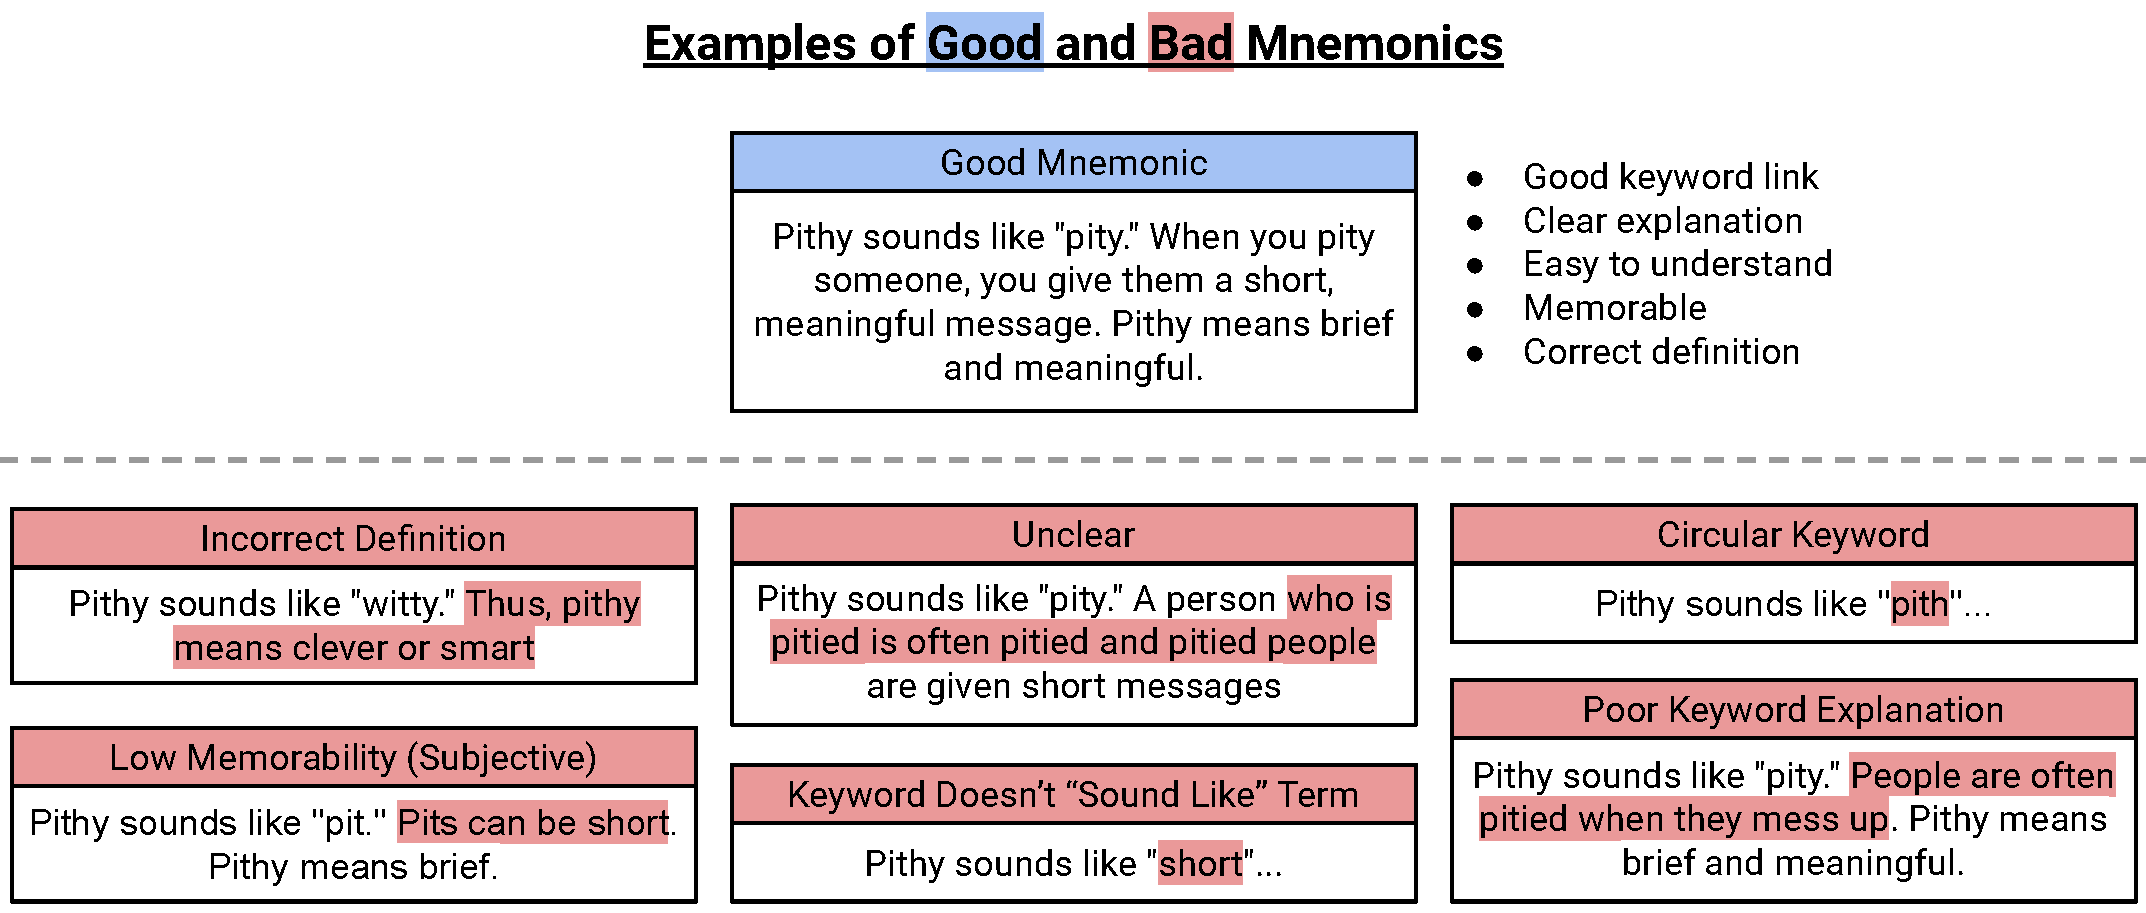
\includegraphics[width=\linewidth]{figures/good_bad_mnemonics.pdf}
%   \caption{Non-exhausitive list of characteristics of a good mnemonic, inferred from \citetext{\citealp{BalepurSMART2024}; \citealp{CamposUSING2011}; \citealp{luExplorationMnemonicsESL2015}; \citealp{SariogluUSE2024}}.}
%   \label{fig:good-bad-mnemonics}
% \end{figure*}

% Define custom colors


% Define custom box styles
\tcbset{
    goodbox/.style={
        colback=goodlight,
        colframe=goodgreen,
        fonttitle=\bfseries\color{white},
        coltitle=white,
        colbacktitle=goodgreen,
        enhanced,
        attach boxed title to top center={yshift=-1mm},
        boxed title style={sharp corners},
        top=2mm,
    },
    badbox/.style={
        colback=badlight,
        colframe=badred,
        fonttitle=\bfseries\color{white},
        coltitle=white,
        colbacktitle=badred,
        enhanced,
        attach boxed title to top center={yshift=-1mm},
        boxed title style={sharp corners},
        top=2mm,
    }
}

% Start the figure environment
\begin{figure*}[htb]
\centering
\footnotesize
% First row - Good mnemonic + characteristics
\begin{minipage}{0.66\textwidth}
    \begin{tcolorbox}[goodbox, title=Good Mnemonic]
        \textcolor{red}{\textbf{preposterous}}: \textcolor{goodgreen}{comes from pre- ("before") + post ("after") + -ous}, meaning reversed or absurd. \textcolor{orange}{An event cannot happen both pre- (before) and post- (after) to us, it is prespoterous!}
    \end{tcolorbox}
\end{minipage}
\hspace{0.5em}
\begin{minipage}{0.3\textwidth}
    \begin{itemize}[leftmargin=*, nosep]
        \item \vocab is used correctly in \mnem
        \item Clear \assoc linking \vocab and \mnem
        \item Strong \assoc
        \item \mnem uses similar or lower vocabulary than \vocab
        \item \mnem is memorable
    \end{itemize}
\end{minipage}

\vspace{0.3cm}

% Second row - 3 bad mnemonics
\begin{minipage}{0.33\textwidth}
    \begin{tcolorbox}[badbox, title=Incorrect Definition]
        Preposterous means very important or significant.
    \end{tcolorbox}
\end{minipage}%
\begin{minipage}{0.33\textwidth}
    \begin{tcolorbox}[badbox, title=Circular Association]
        Preposterous sounds like preposterous.
    \end{tcolorbox}
\end{minipage}%
\begin{minipage}{0.33\textwidth}
    \begin{tcolorbox}[badbox, title=Weak Association]
        Preposterous sounds like prosperous. Preposterous people usually make prosperous business decisions.
    \end{tcolorbox}
\end{minipage}

\vspace{0.3cm}

% Third row - 3 more bad mnemonics
\begin{minipage}{0.33\textwidth}
    \begin{tcolorbox}[badbox, title=Difficult Vocabulary]
        Preposterous means ludicrously implausible or contrary to conventional hierarchies of logical induction.
    \end{tcolorbox}
\end{minipage}%
\begin{minipage}{0.33\textwidth}
    \begin{tcolorbox}[badbox, title=Too Abstract]
        Preposterous describes logical fallacies where the premise negates itself through temporal displacement.
    \end{tcolorbox}
\end{minipage}%
\begin{minipage}{0.33\textwidth}
    \begin{tcolorbox}[badbox, title=Offensive Content]
        Preposterous contains "post" which reminds me of [inappropriate culturally-specific reference].
    \end{tcolorbox}
\end{minipage}

\caption{Characteristics of good mnemonics, and examples of bad mnemonics. We propose VAM/VEM model, where a good mnemonic must have three components: \vocabulary (\vocab), \association (\assoc) (or explanation ($e$)), and \mnemonic (\mnem), with characteristics listed above. These characteristics are also available in list (\Cref{app:mnemonic-characteristics})}
\label{fig:good-bad-mnemonics}
\end{figure*}


Mnemonic devices are mental techniques that enhance memory through meaningful associations between new information and pre-existing knowledge \citep{pressleyMnemonicKeywordMethod1982,PintrichROLE2002}. For vocabulary acquisition, the keyword method has been widely studied. The method involves creating acoustically or orthographically similar keywords to the target vocabulary, followed by an association between these keywords and the word's meaning \citep{atkinsonApplicationMnemonicKeyword1975}.

While the keyword method has shown effectiveness in classroom and laboratory contexts, its success often relies on several factors. It enhances recall for concrete vocabulary, since learners can easily create mental imagery for it \citep{schwanenflugelContextAvailabilityRecall1992,wangKeywordMnemonicRetention1992}. However, its effectiveness diminishes for abstract vocabulary \citep{fothMnemonicTechniqueEffectiveness1973,CamposLIMITATIONS2003},  experienced language learners with high proficiency \citep{vanhellKeywordMnemonicsRote1997,CamposUSING2011}, and mnemonics not created by the learners themselves \citep{camposImportanceKeywordGenerationMethod2004a,madanExploringWordMemorability2021}, sometimes with longer recall and lower retention than rote learning.

More linguistically sophisticated approaches, such as etymology-based mnemonics, could provide deeper encoding and potentially stronger retention for abstract vocabulary \citep{ piersonUsingEtymologyClassroom1989,akarslanEffectsTeachingWord2019, gangavarapuUsingEtymologyVocabulary2024}. These approaches leverage morphological, etymological, and semantic properties of words, creating more meaningful associations that align with how language is naturally structured \citep{zhangApplicationEtymologySemantic2013}.

Psycholinguistics offers other insights into factors that enhance mnemonic recall by investigating memorability, how easily information is remembered, based on its inherent characteristics and the context in which it appears. Mnemonics are more effective when they incorporate animate entities, indicators of potential usefulness, and concrete visual imagery \citep{schwanenflugelContextAvailabilityRecall1992,ledingAdaptiveMemoryAnimacy2019,madanExploringWordMemorability2021}. Moreover, emotionally charged associations produce stronger memory traces than neutral ones \citep{altarribaConcretenessContextAvailability1999}, and mnemonics that involve deeper linguistic analysis yield more robust recall \citep{rankinAgePresentationRate1983, SariogluUSE2024}. These findings underscore the importance of both the content and the cognitive strategies applied during encoding in achieving optimal memorability.

We explore these principles in our work, focusing on how LLMs can generate mnemonics that incorporate good characteristics (\Cref{fig:good-bad-mnemonics}) and leverage linguistic features (\Cref{tab:linguistic-features}).

\subsection{LLMs: linguistic competence, reasoning, and creativity} \label{sec:llm-linguistic-competence}

Significant advancements have been made in enhancing the reasoning capabilities of large language models (LLMs), particularly in mathematical and scientific domains where problems have unique correct answers. Several prompting techniques were introduced to make LLMs learn from demonstrations (or "shots") or produce explicit step-by-step thinking processes to improve their reasoning, notably few-shot prompting \citep{brownFewShotLearners2020}, chain-of-thought (CoT) \citep{weiChainofThoughtPromptingElicits2022}, self-consistency \citep{wangSelfConsistencyImprovesChain2022}, zero-shot reasoning \citep{kojimaZeroShotReasoners2022}, analogical reasoning (automated few-shot CoT) \citep{YasunagaLLMAnalogicalReasoners2023}. Post-training techniques such as reinforcement learning from human feedback (RLHF) \citep{ouyangRLHF2022} and CoT data \citep{DeepSeek-AIDEEPSEEKR12025} further endows LLMs with instruction-following and reasoning capabilities. However, LLMs still struggle with complex reasoning tasks that require multiple steps, abstract thinking \citep{weiChainofThoughtPromptingElicits2022} or low-frequency knowledge \citep{kandpalLongTailKnowledge2023,sunHeadtoTailHowKnowledgeable2024}.

The ability to use and reason through languages falls into the categories of long-tail knowledge and abstract reasoning. Recent studies have explored LLMs' linguistic competence, defined as their ability to understand and apply language rules and patterns \citep{waldisHOLMES2024}. LLMs typically perform better on formal linguistic competence tasks, such as morphology and syntax, than on functional linguistic competence tasks, such as semantics, discourse \citep{KhoujaLINGOLYTOO2025} or phonology \citep{suvarnaPhonologyBenchEvaluatingPhonological2024}. Their competence is influenced by model architecture, with encoder-based models often outperforming decoder-only models, and larger models generally showing better linguistic understanding \citep{waldisHOLMES2024}. Instruction tuning could improve performance on linguistic tasks, though sometimes at the expense of deeper language understanding \citep{waldisHOLMES2024,yinDidYouRead2023}.

LLMs can also perform inductive multilingual reasoning, primarily demonstrated through inferring rules in linguistic puzzles as seen in International Olympiad in Linguistics, especially when provided with analogical demonstrations \citep{RamjiINDUCTIVE2024}. However, its reasoning remains inconsistent, with performance varying across minor problem perturbations, suggesting that it may not fully understand the underlying linguistic principles and memorize it \citep{RamjiINDUCTIVE2024,KhoujaLINGOLYTOO2025}. This inconsistency is also observed in mathematical reasoning tasks, where LLMs can produce correct answers but often fail to provide coherent explanations \citep{weiChainofThoughtPromptingElicits2022}.

For mnemonic generation specifically, previous work has explored using LLMs for automated keyword mnemonic generation \citep{savvaTransPhonerAutomatedMnemonic2014,OzbalAUTOMATION2014,LeeSMARTPHONE2023,LeeEXPLORING2024,BalepurSMART2024}, but these approaches have primarily focused on phonetic similarity rather than leveraging the broader linguistic knowledge embedded in LLMs. Our work extends these efforts by exploring how LLMs can use linguistic reasoning abilities to analyze multiple linguistic features, choose the most relevant ones to generate mnemonic devices.
